% A3 ten-figures × A–D float carrier (campaign research-20260810-ten-figures)
% Does NOT replace the 7-figure journal spine in manuscript.tex — compliance vehicle only.
\documentclass[11pt]{article}
\usepackage[margin=0.9in]{geometry}
\usepackage{graphicx}
\usepackage{booktabs}
\title{A3 ten-figures float carrier (spine-preserving)}
\author{Zeyu Fu}
\date{2026-08-10}
\begin{document}
\maketitle
\noindent\textit{Companion to} \texttt{manuscript.tex}. Reclaims three SI faces (ex-F2/F6/F10) so the carrier has $\geq$10 four-panel floats without mutating the locked 7-figure main spine. Assets from \texttt{scripts/R/make\_four\_panel\_all.R} + committed \texttt{figures/plotdata}.

\begin{figure}[p]\centering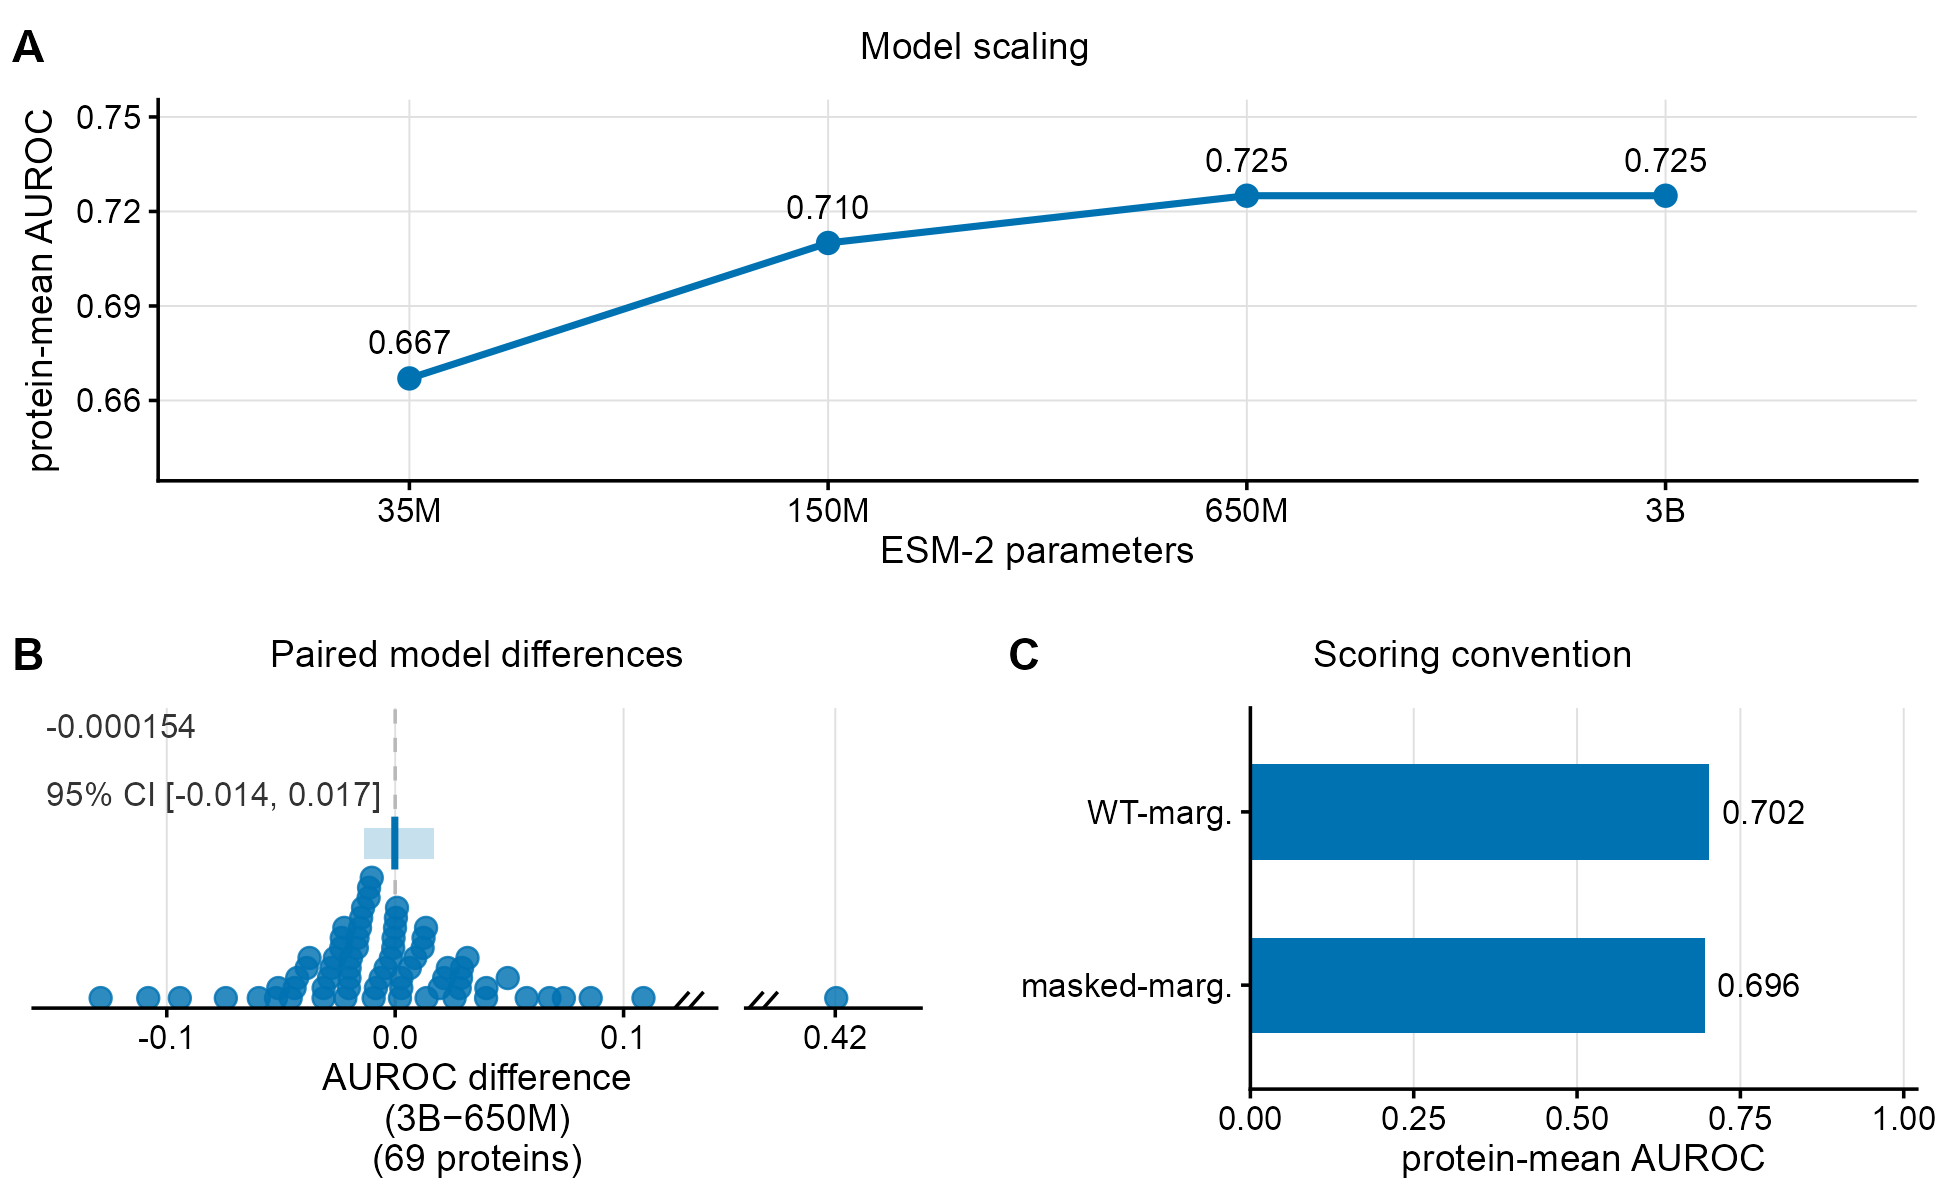
\includegraphics[width=\textwidth,height=0.82\textheight,keepaspectratio]{figures/F1_scale_plateau.png}
\caption{\textbf{Fig 1.} Scale plateau. (A) AUROC vs size. (B) Discriminating protein count. (C) Stepwise $\Delta$AUROC. (D) Fraction discriminating.}\label{fig:f1}\end{figure}

\begin{figure}[p]\centering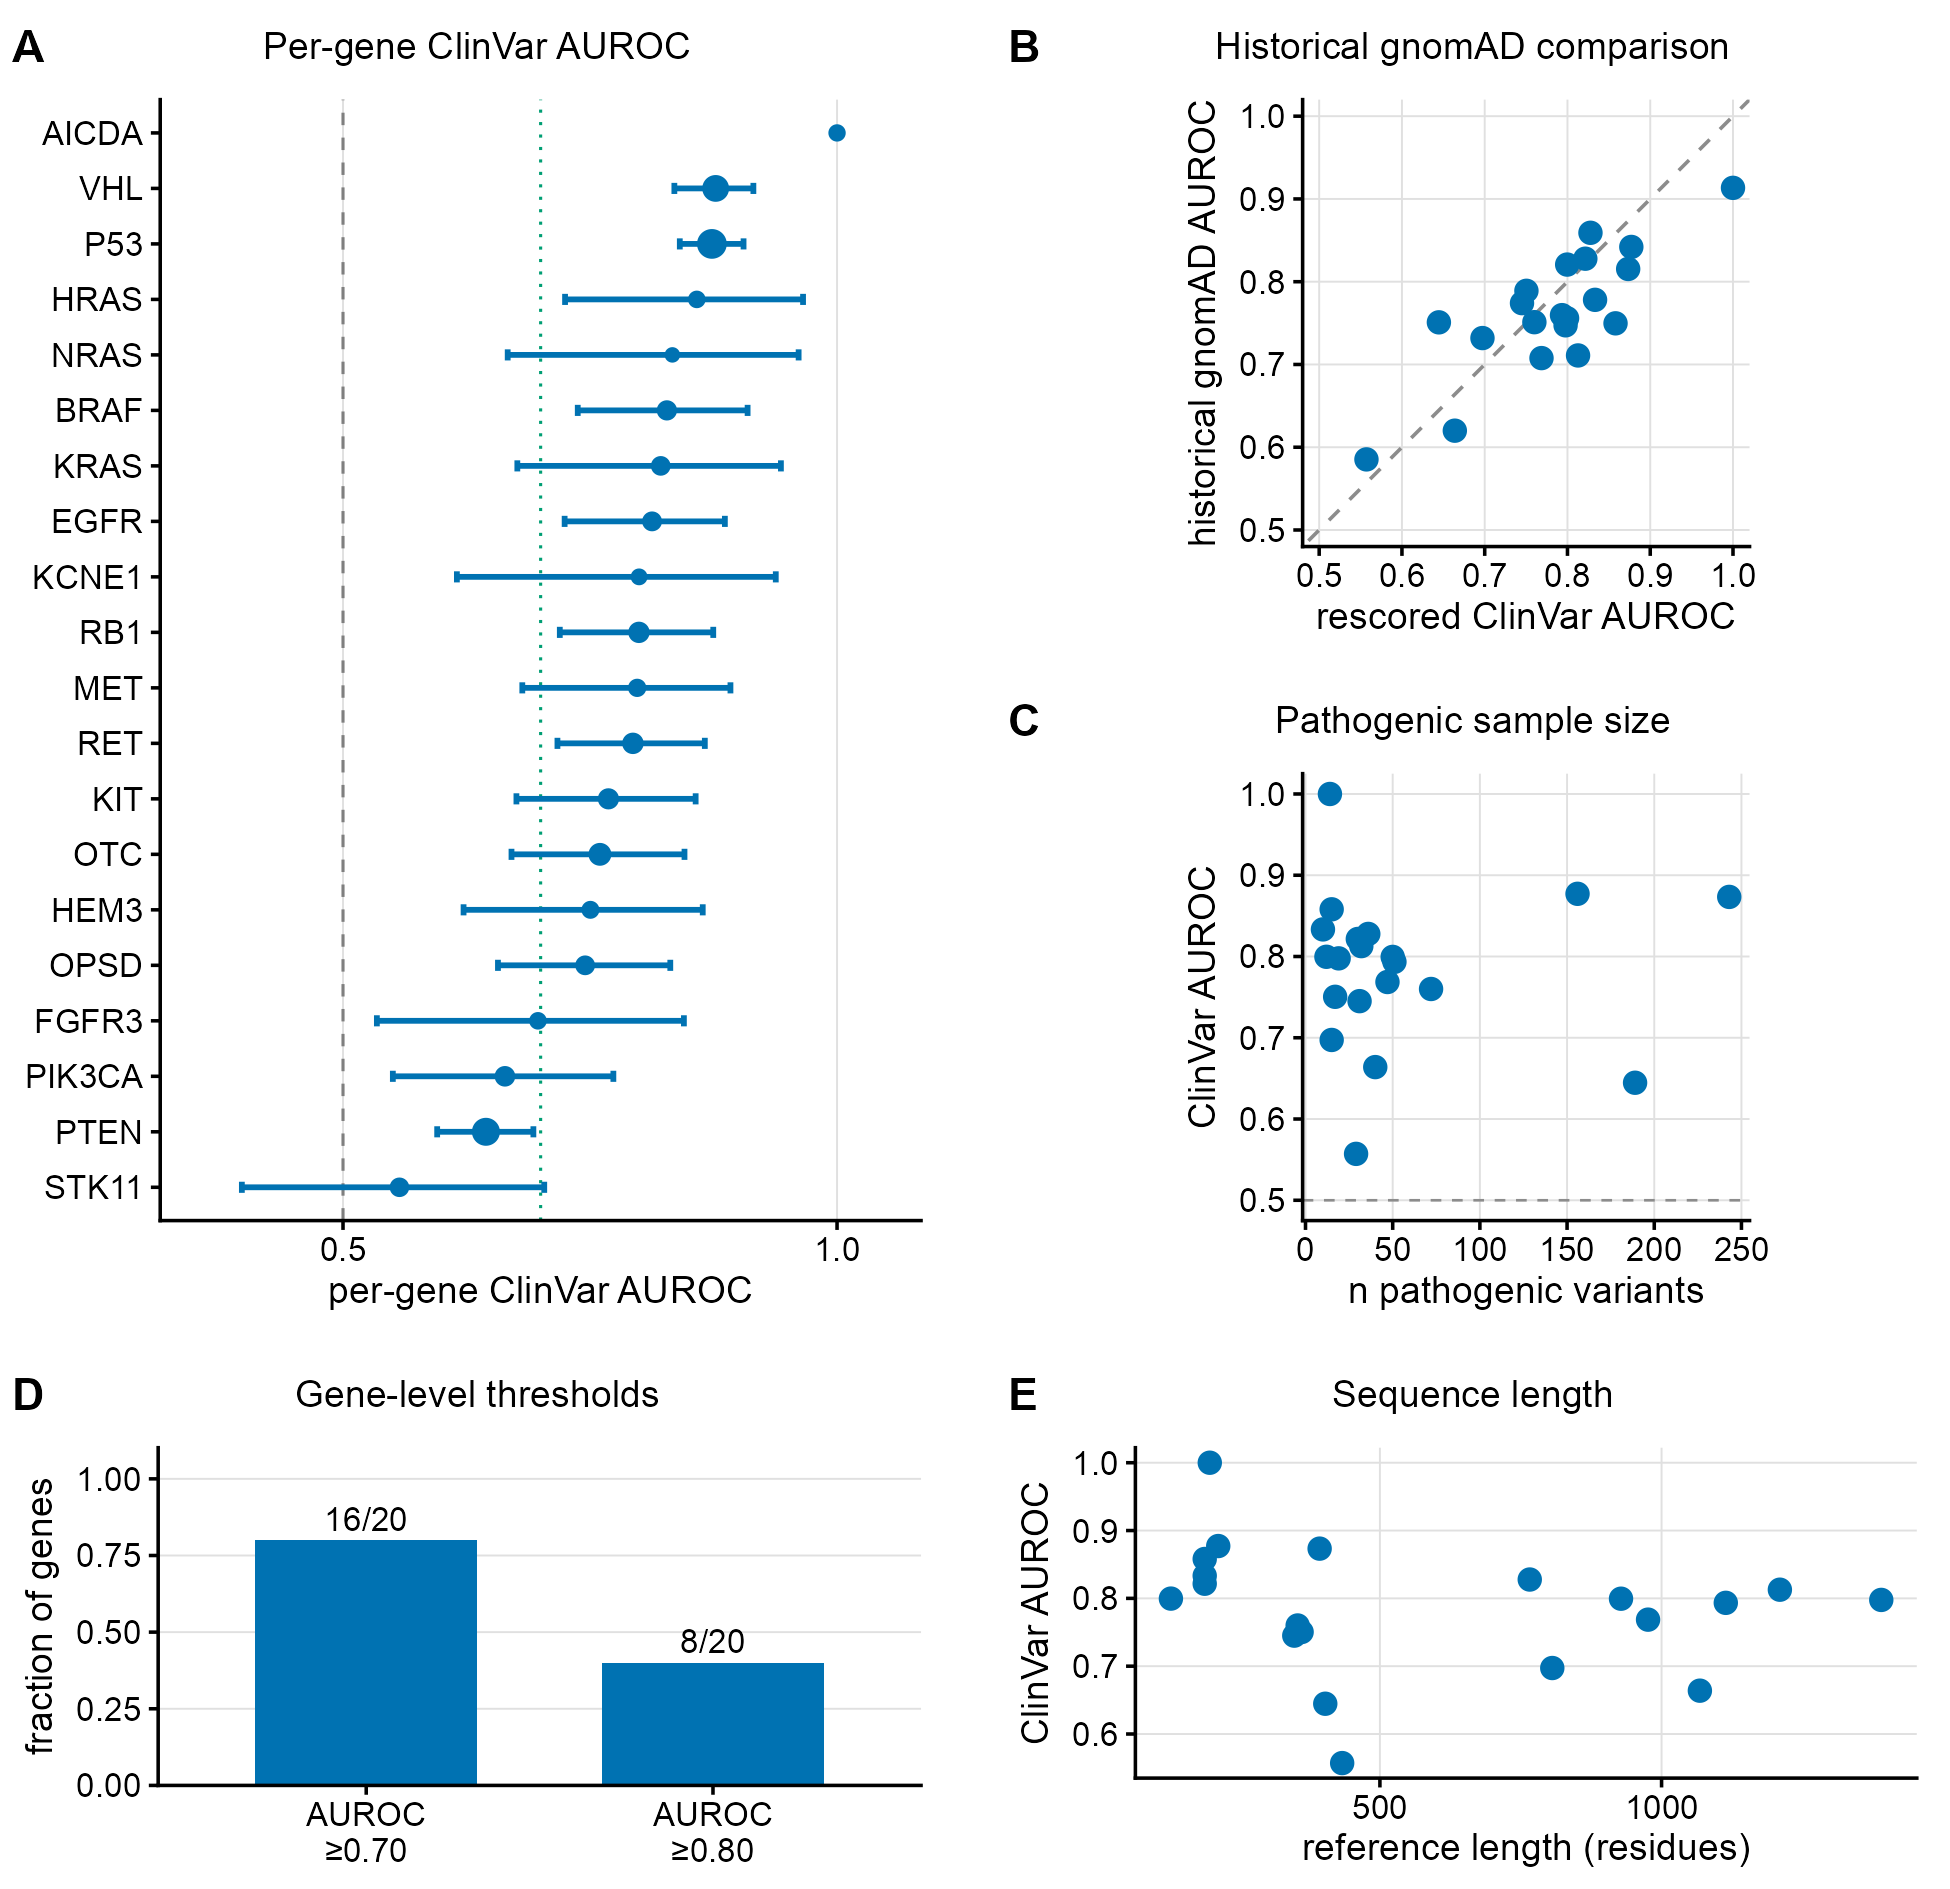
\includegraphics[width=\textwidth,height=0.82\textheight,keepaspectratio]{figures/F3_clinvar_forest.png}
\caption{\textbf{Fig 3.} ClinVar transfer. (A) Per-gene forest. (B) ClinVar vs gnomAD. (C) AUROC vs $n$. (D) Threshold fractions.}\label{fig:f3}\end{figure}

\begin{figure}[p]\centering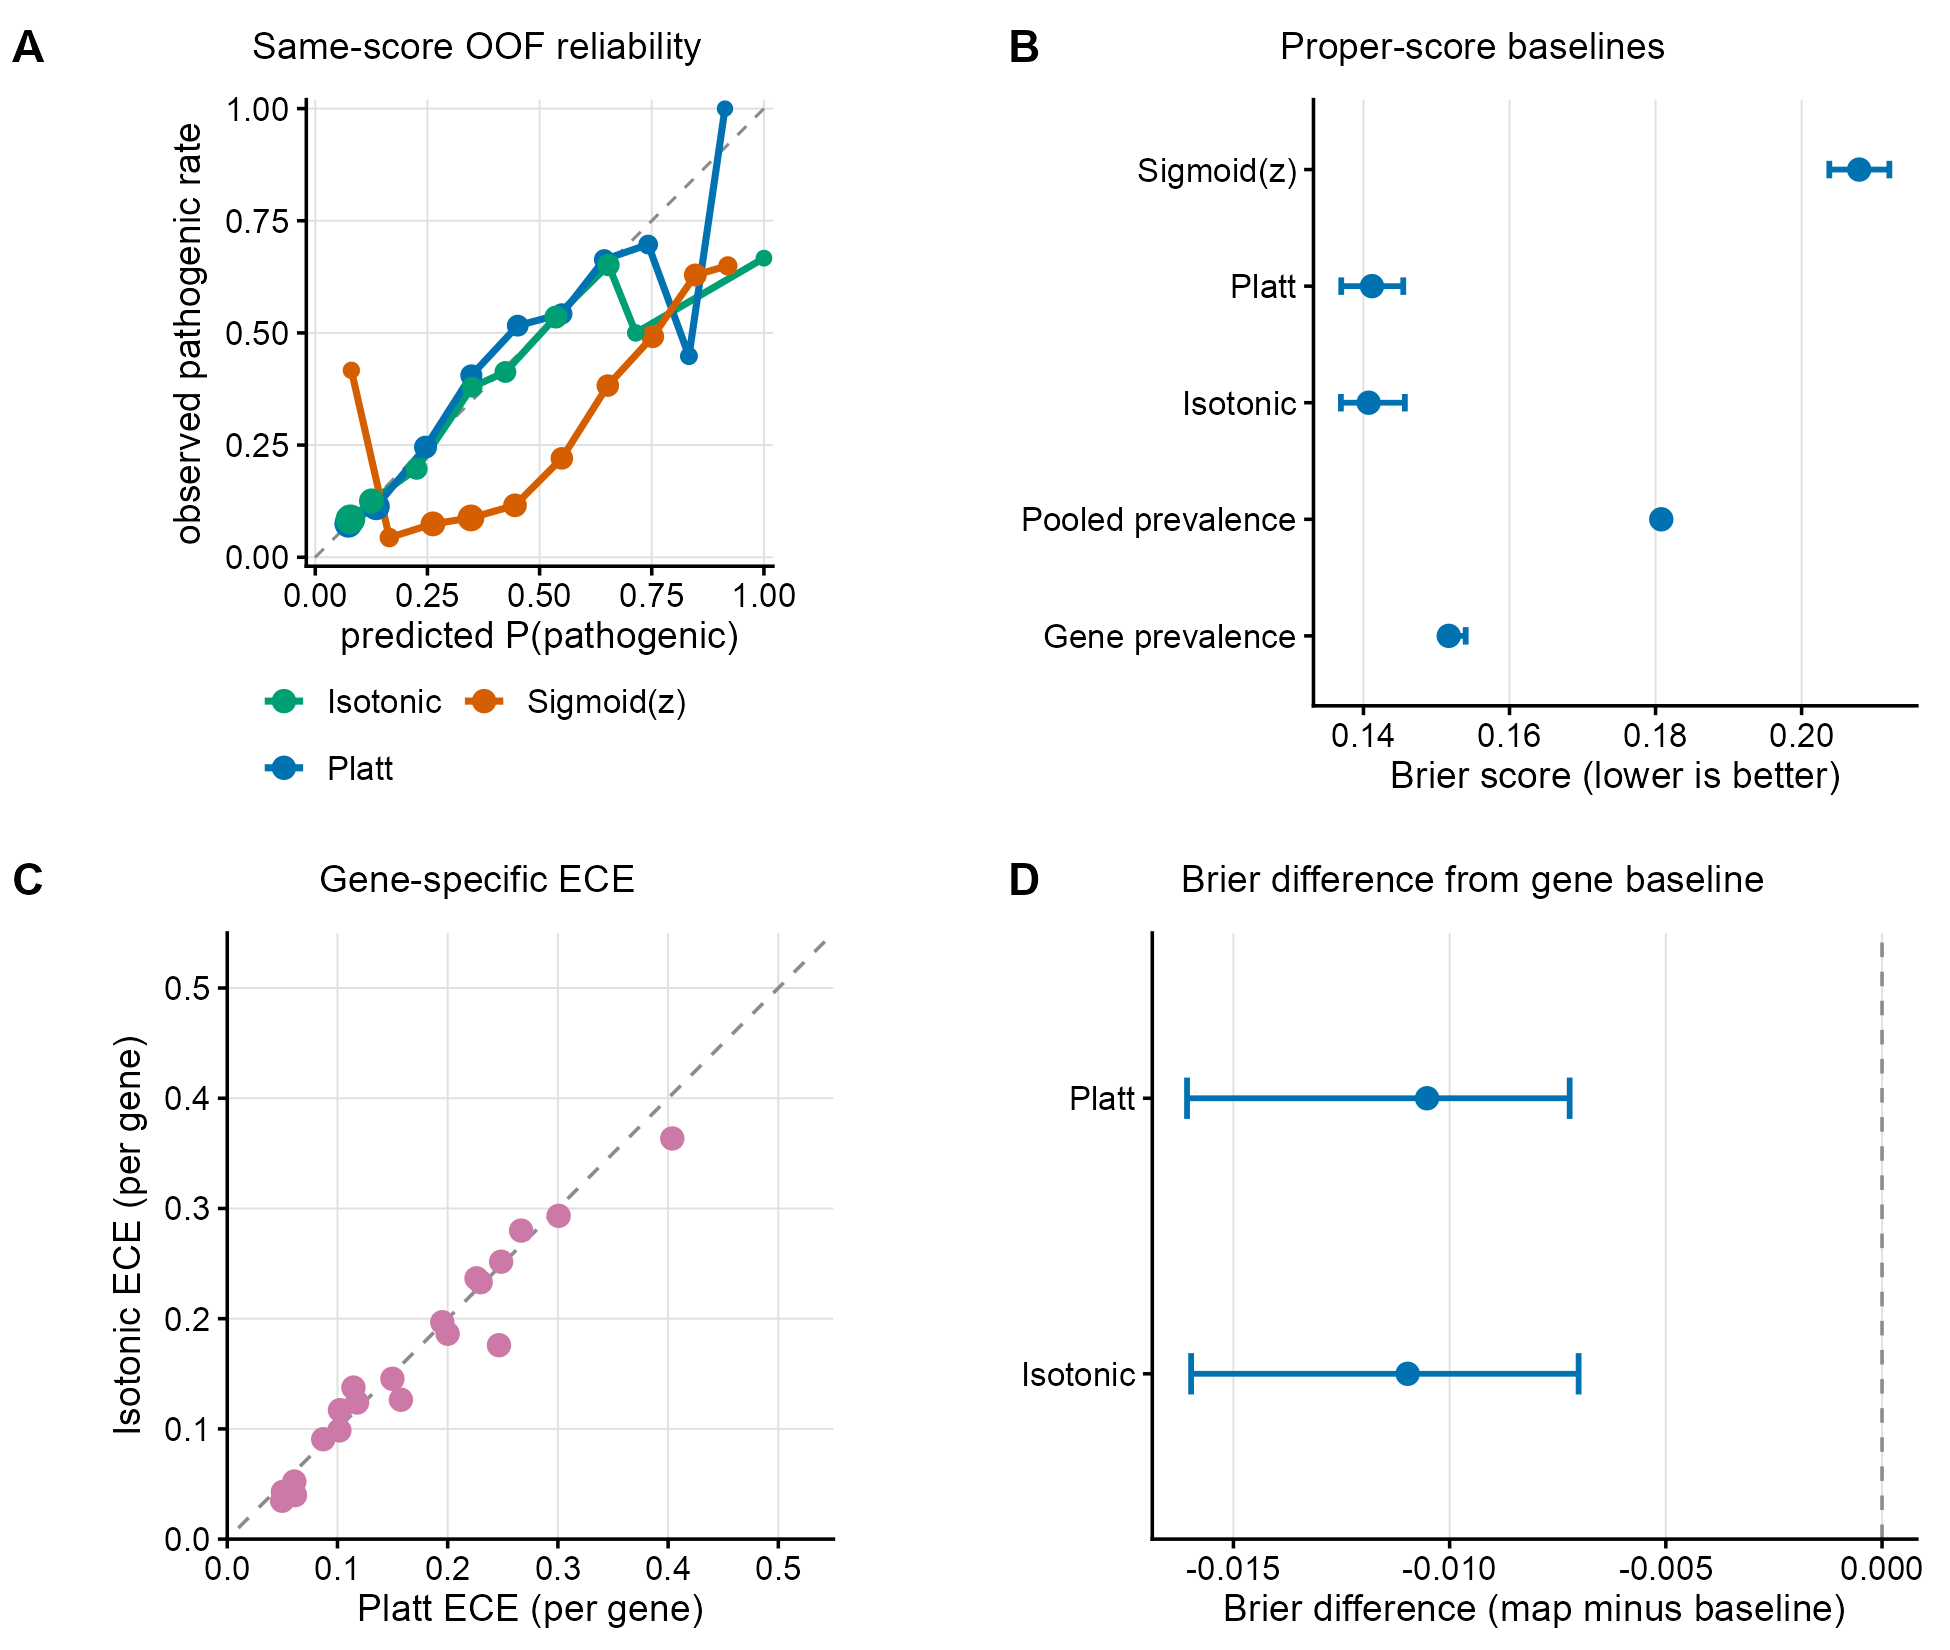
\includegraphics[width=\textwidth,height=0.82\textheight,keepaspectratio]{figures/F4_clinical_calibration.png}
\caption{\textbf{Fig 4.} Clinical calibration. (A) Reliability. (B) Abstention. (C) ESM-2 vs ESM-1v. (D) Pathogenic calls vs coverage.}\label{fig:f4}\end{figure}

\begin{figure}[p]\centering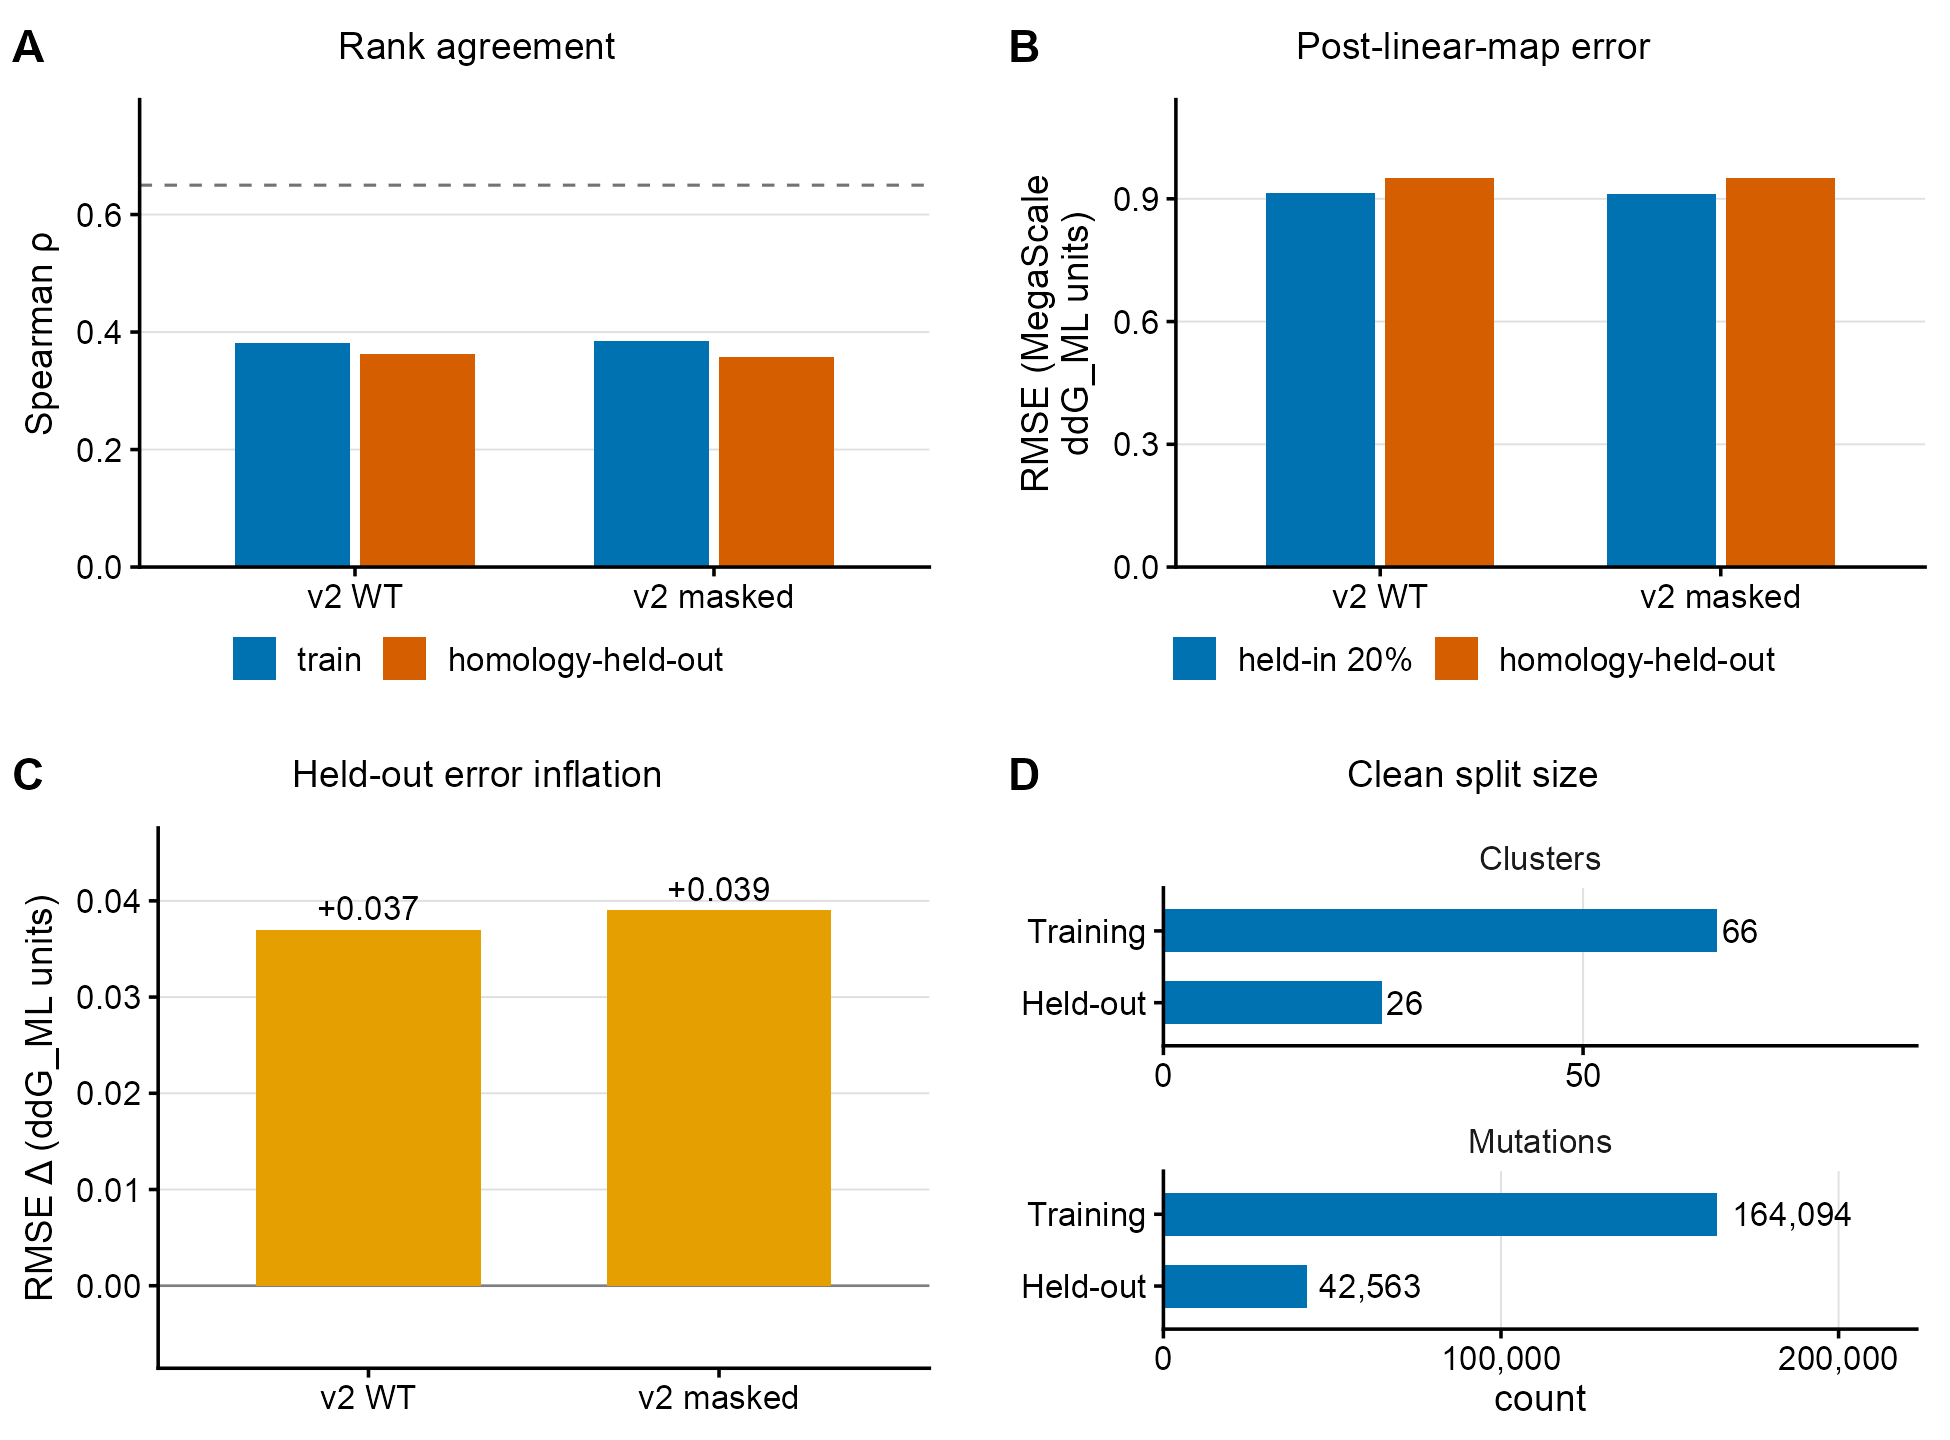
\includegraphics[width=\textwidth,height=0.82\textheight,keepaspectratio]{figures/F5_stability_ddg.png}
\caption{\textbf{Fig 5.} Stability $\Delta\Delta$G. (A) Discrimination train/hold-out. (B) Calibration RMSE. (C) RMSE inflation. (D) Split sizes.}\label{fig:f5}\end{figure}

\begin{figure}[p]\centering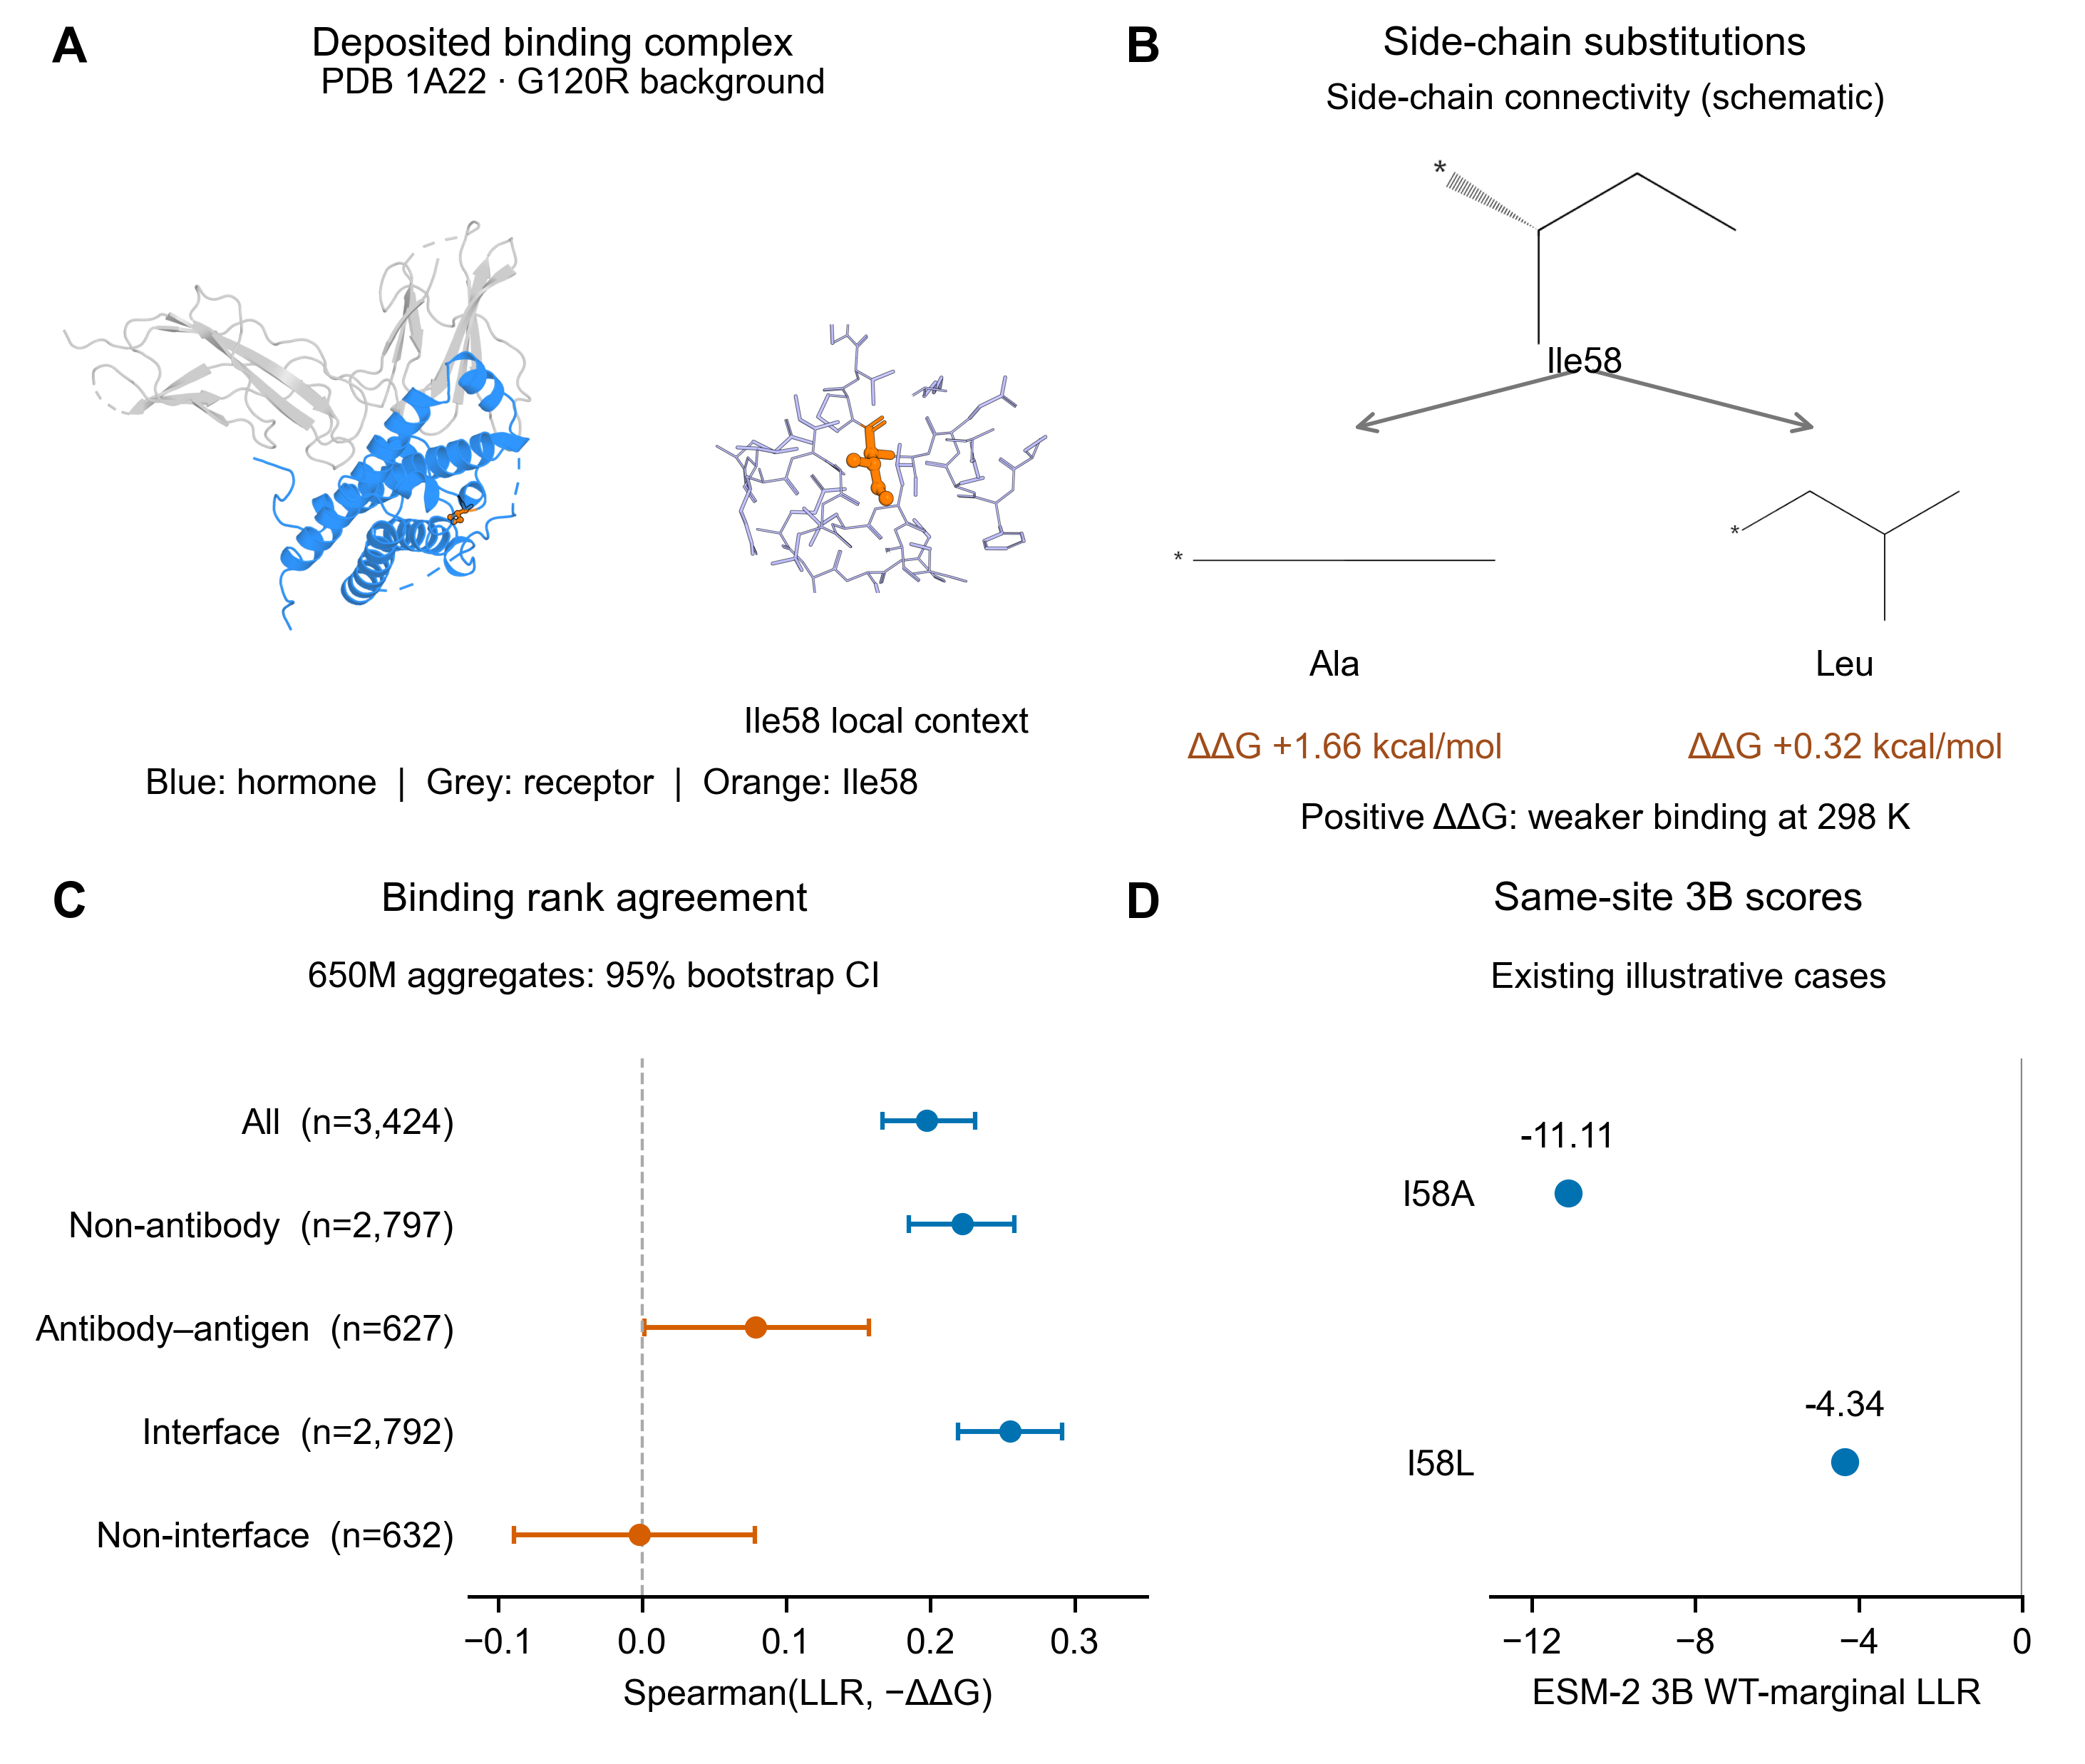
\includegraphics[width=\textwidth,height=0.82\textheight,keepaspectratio]{figures/F7_binding_boundary.png}
\caption{\textbf{Fig 7.} Binding boundary. (A) Spearman by subset. (B) $n$ mutations. (C) CI width. (D) Key contrasts.}\label{fig:f7}\end{figure}

\begin{figure}[p]\centering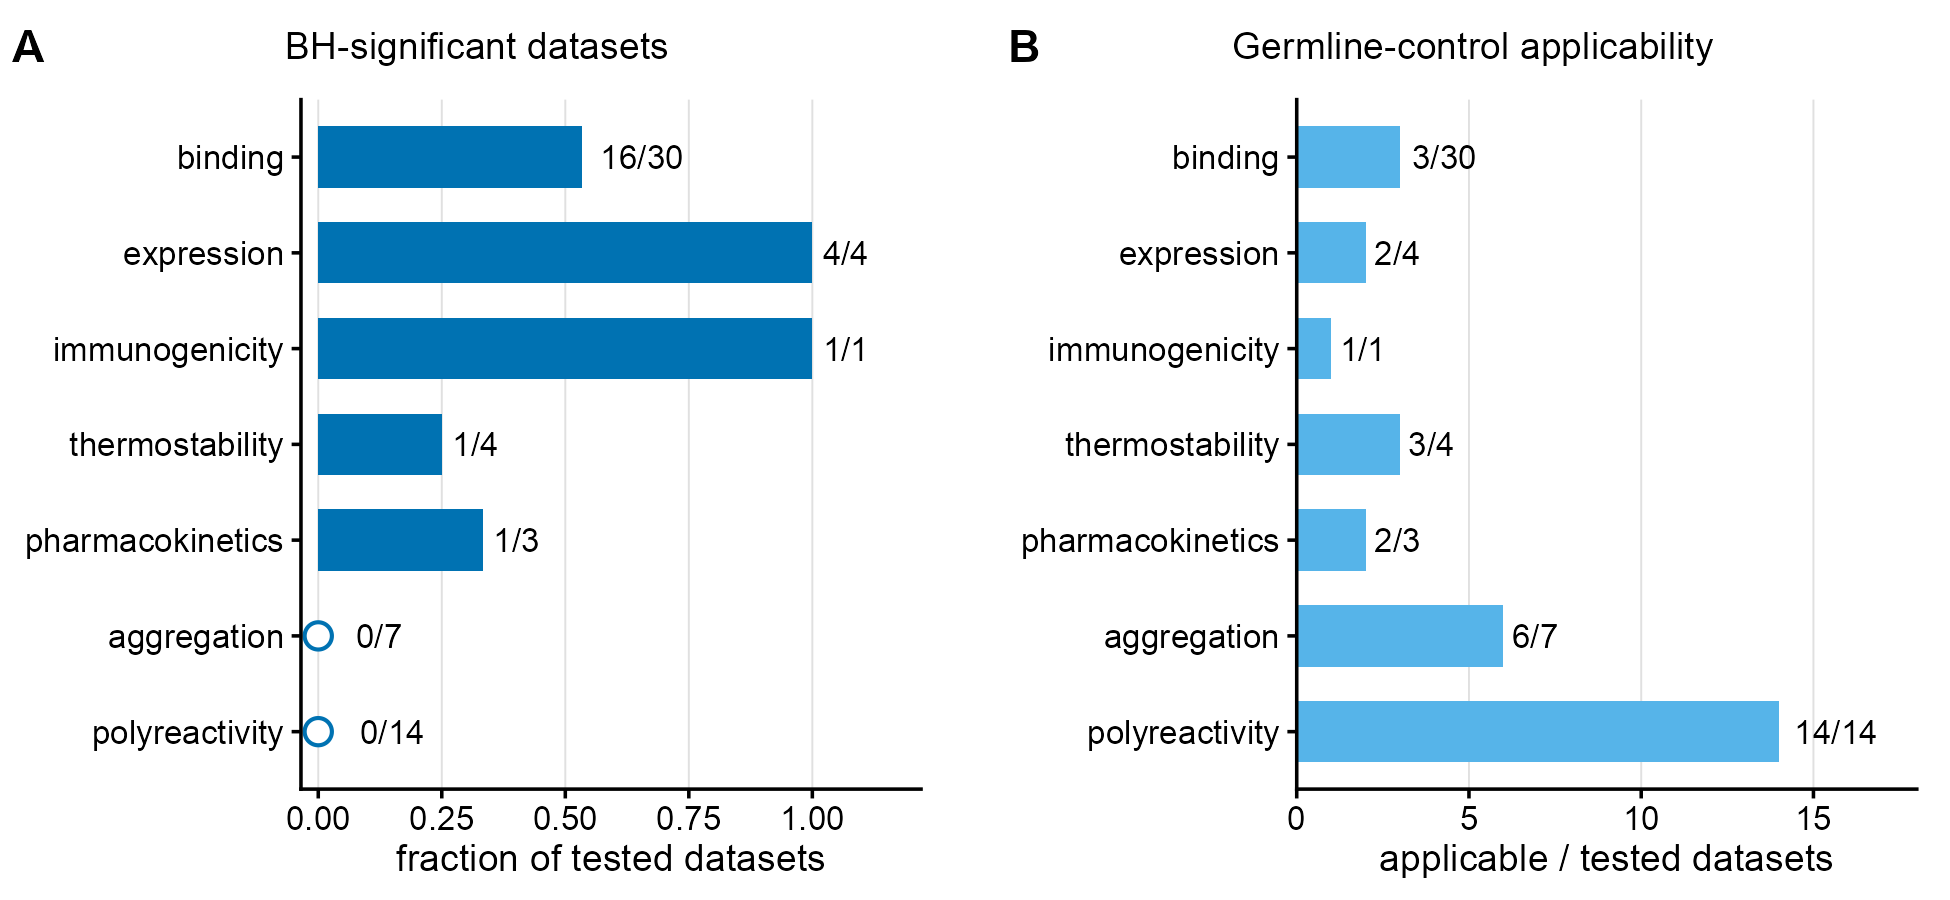
\includegraphics[width=\textwidth,height=0.82\textheight,keepaspectratio]{figures/F8_developability_map.png}
\caption{\textbf{Fig 8.} Developability map. (A) BH-significant fraction. (B) Significant vs $n$. (C) Liability vs non-liability. (D) Multi-germline applicable $n$.}\label{fig:f8}\end{figure}

\begin{figure}[p]\centering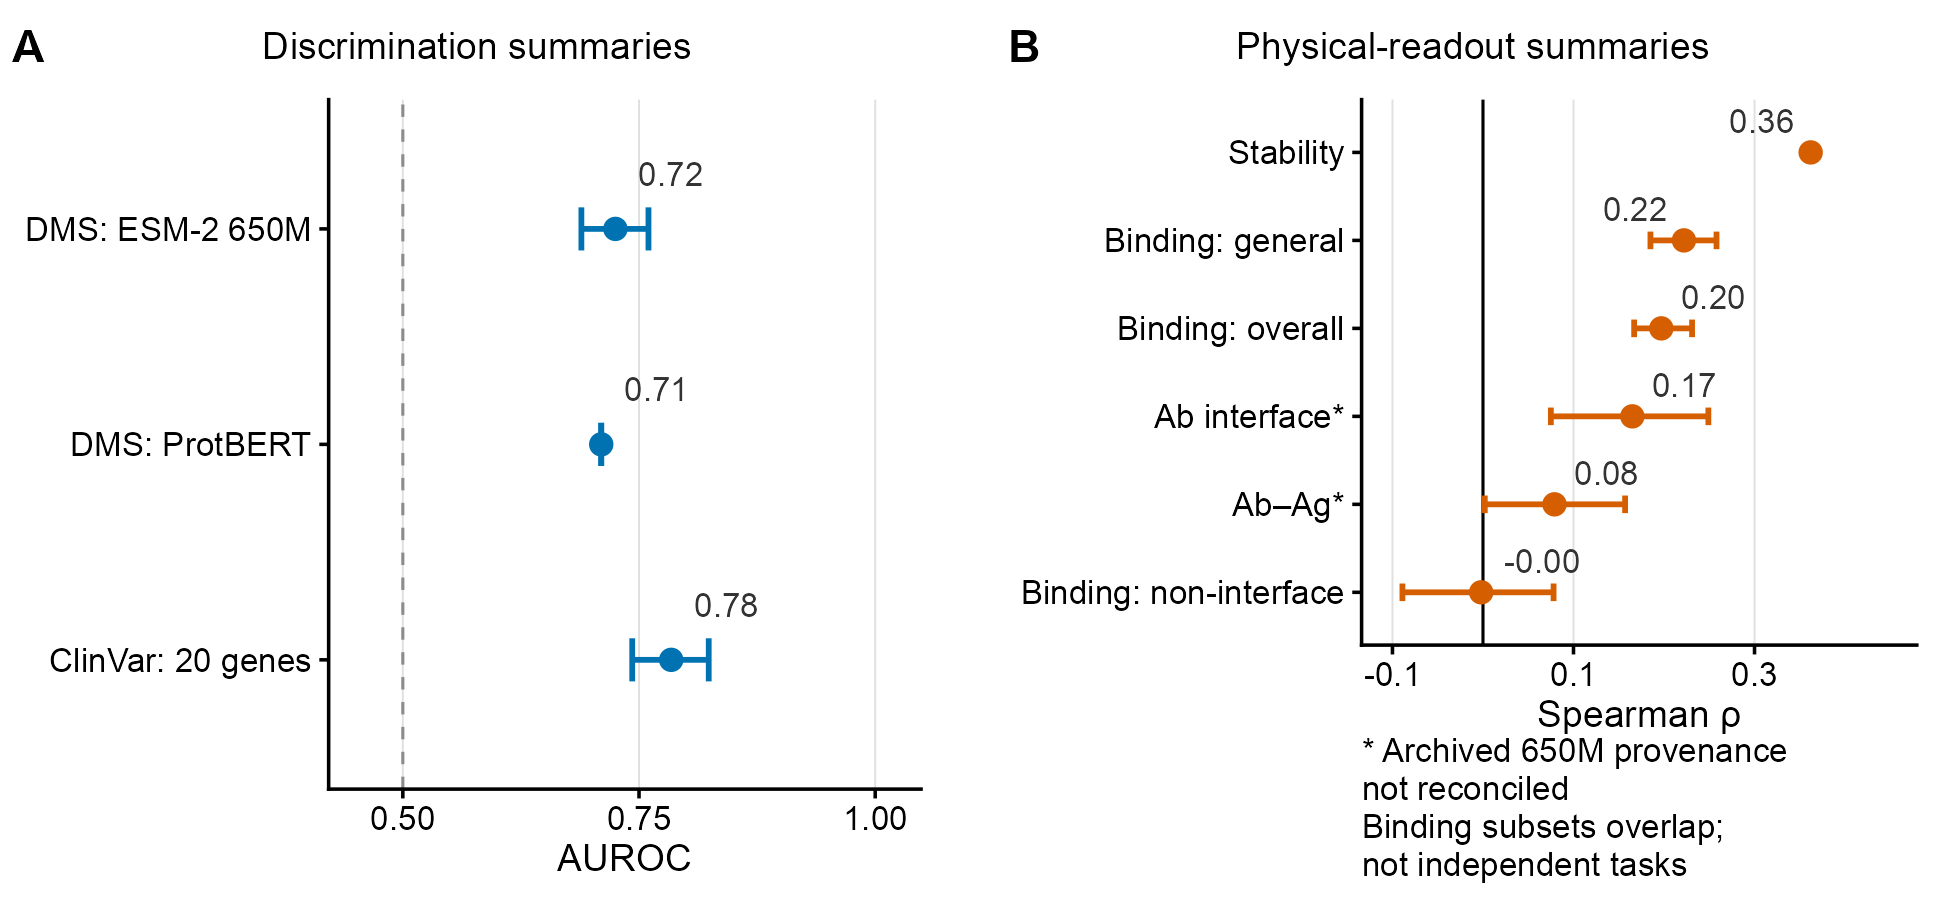
\includegraphics[width=\textwidth,height=0.82\textheight,keepaspectratio]{figures/F11_boundary_atlas.png}
\caption{\textbf{Fig 11.} Boundary atlas. (A) Discrimination tasks. (B) Physical tasks. (C) Cross-axis bars. (D) Hold-vs-collapse summary.}\label{fig:f11}\end{figure}

\begin{figure}[p]\centering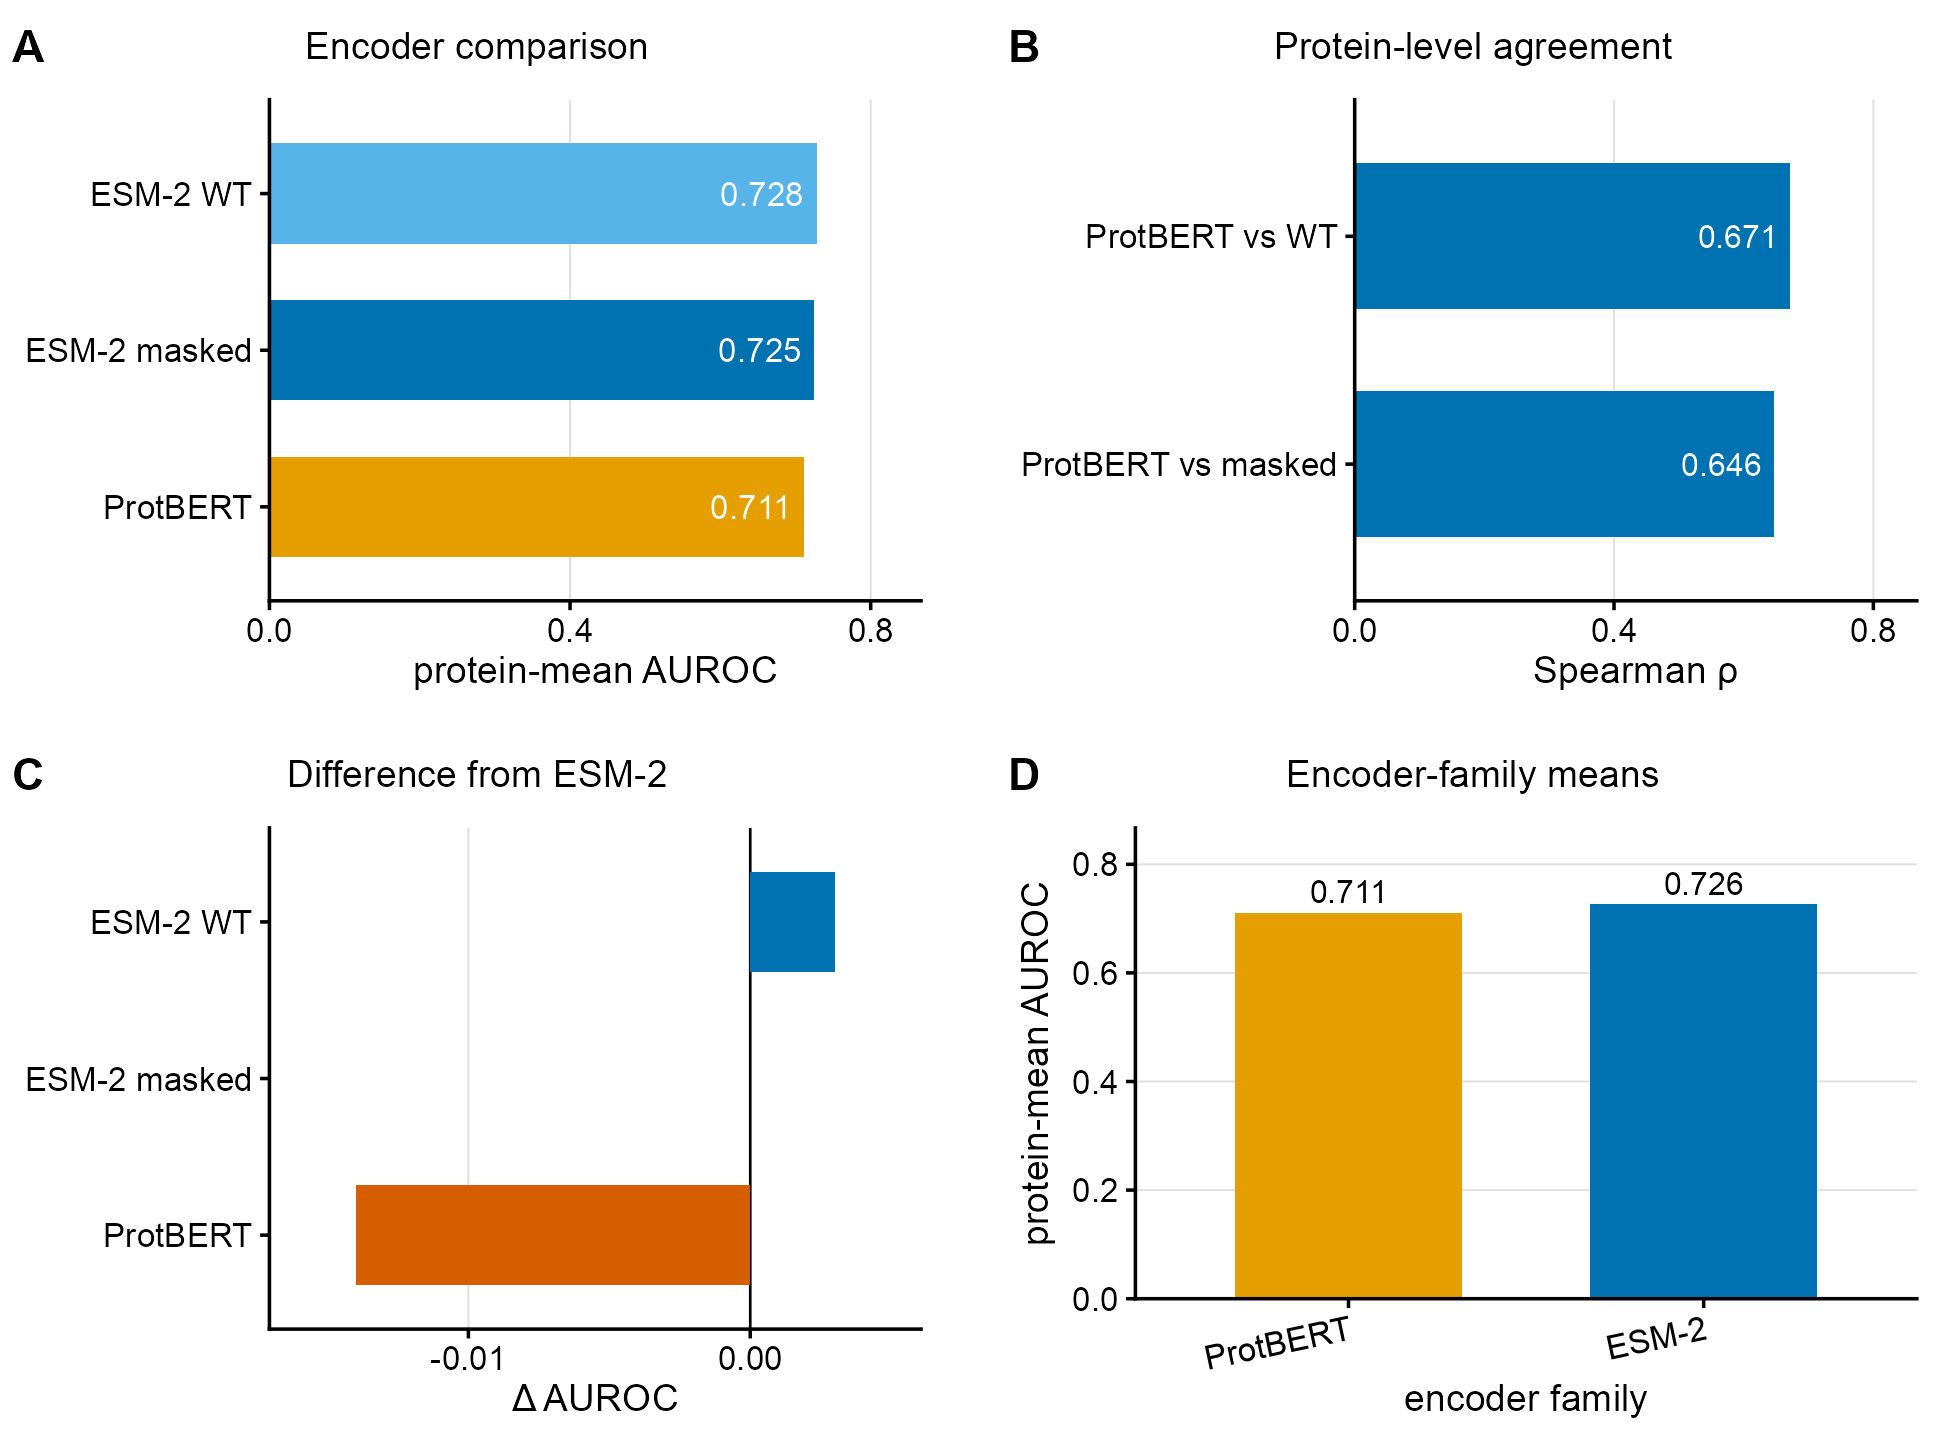
\includegraphics[width=\textwidth,height=0.82\textheight,keepaspectratio]{figures/F2_cross_model.png}
\caption{\textbf{Fig 8$^\dagger$ (promoted SI S6 / ex-F2).} Cross-encoder. (A)~ProtBERT vs ESM-2 AUROC. (B)~Per-protein agreement. (C)~Encoder divergence summary. (D)~Committed score-variant contrast.}\label{fig:f2}\end{figure}

\begin{figure}[p]\centering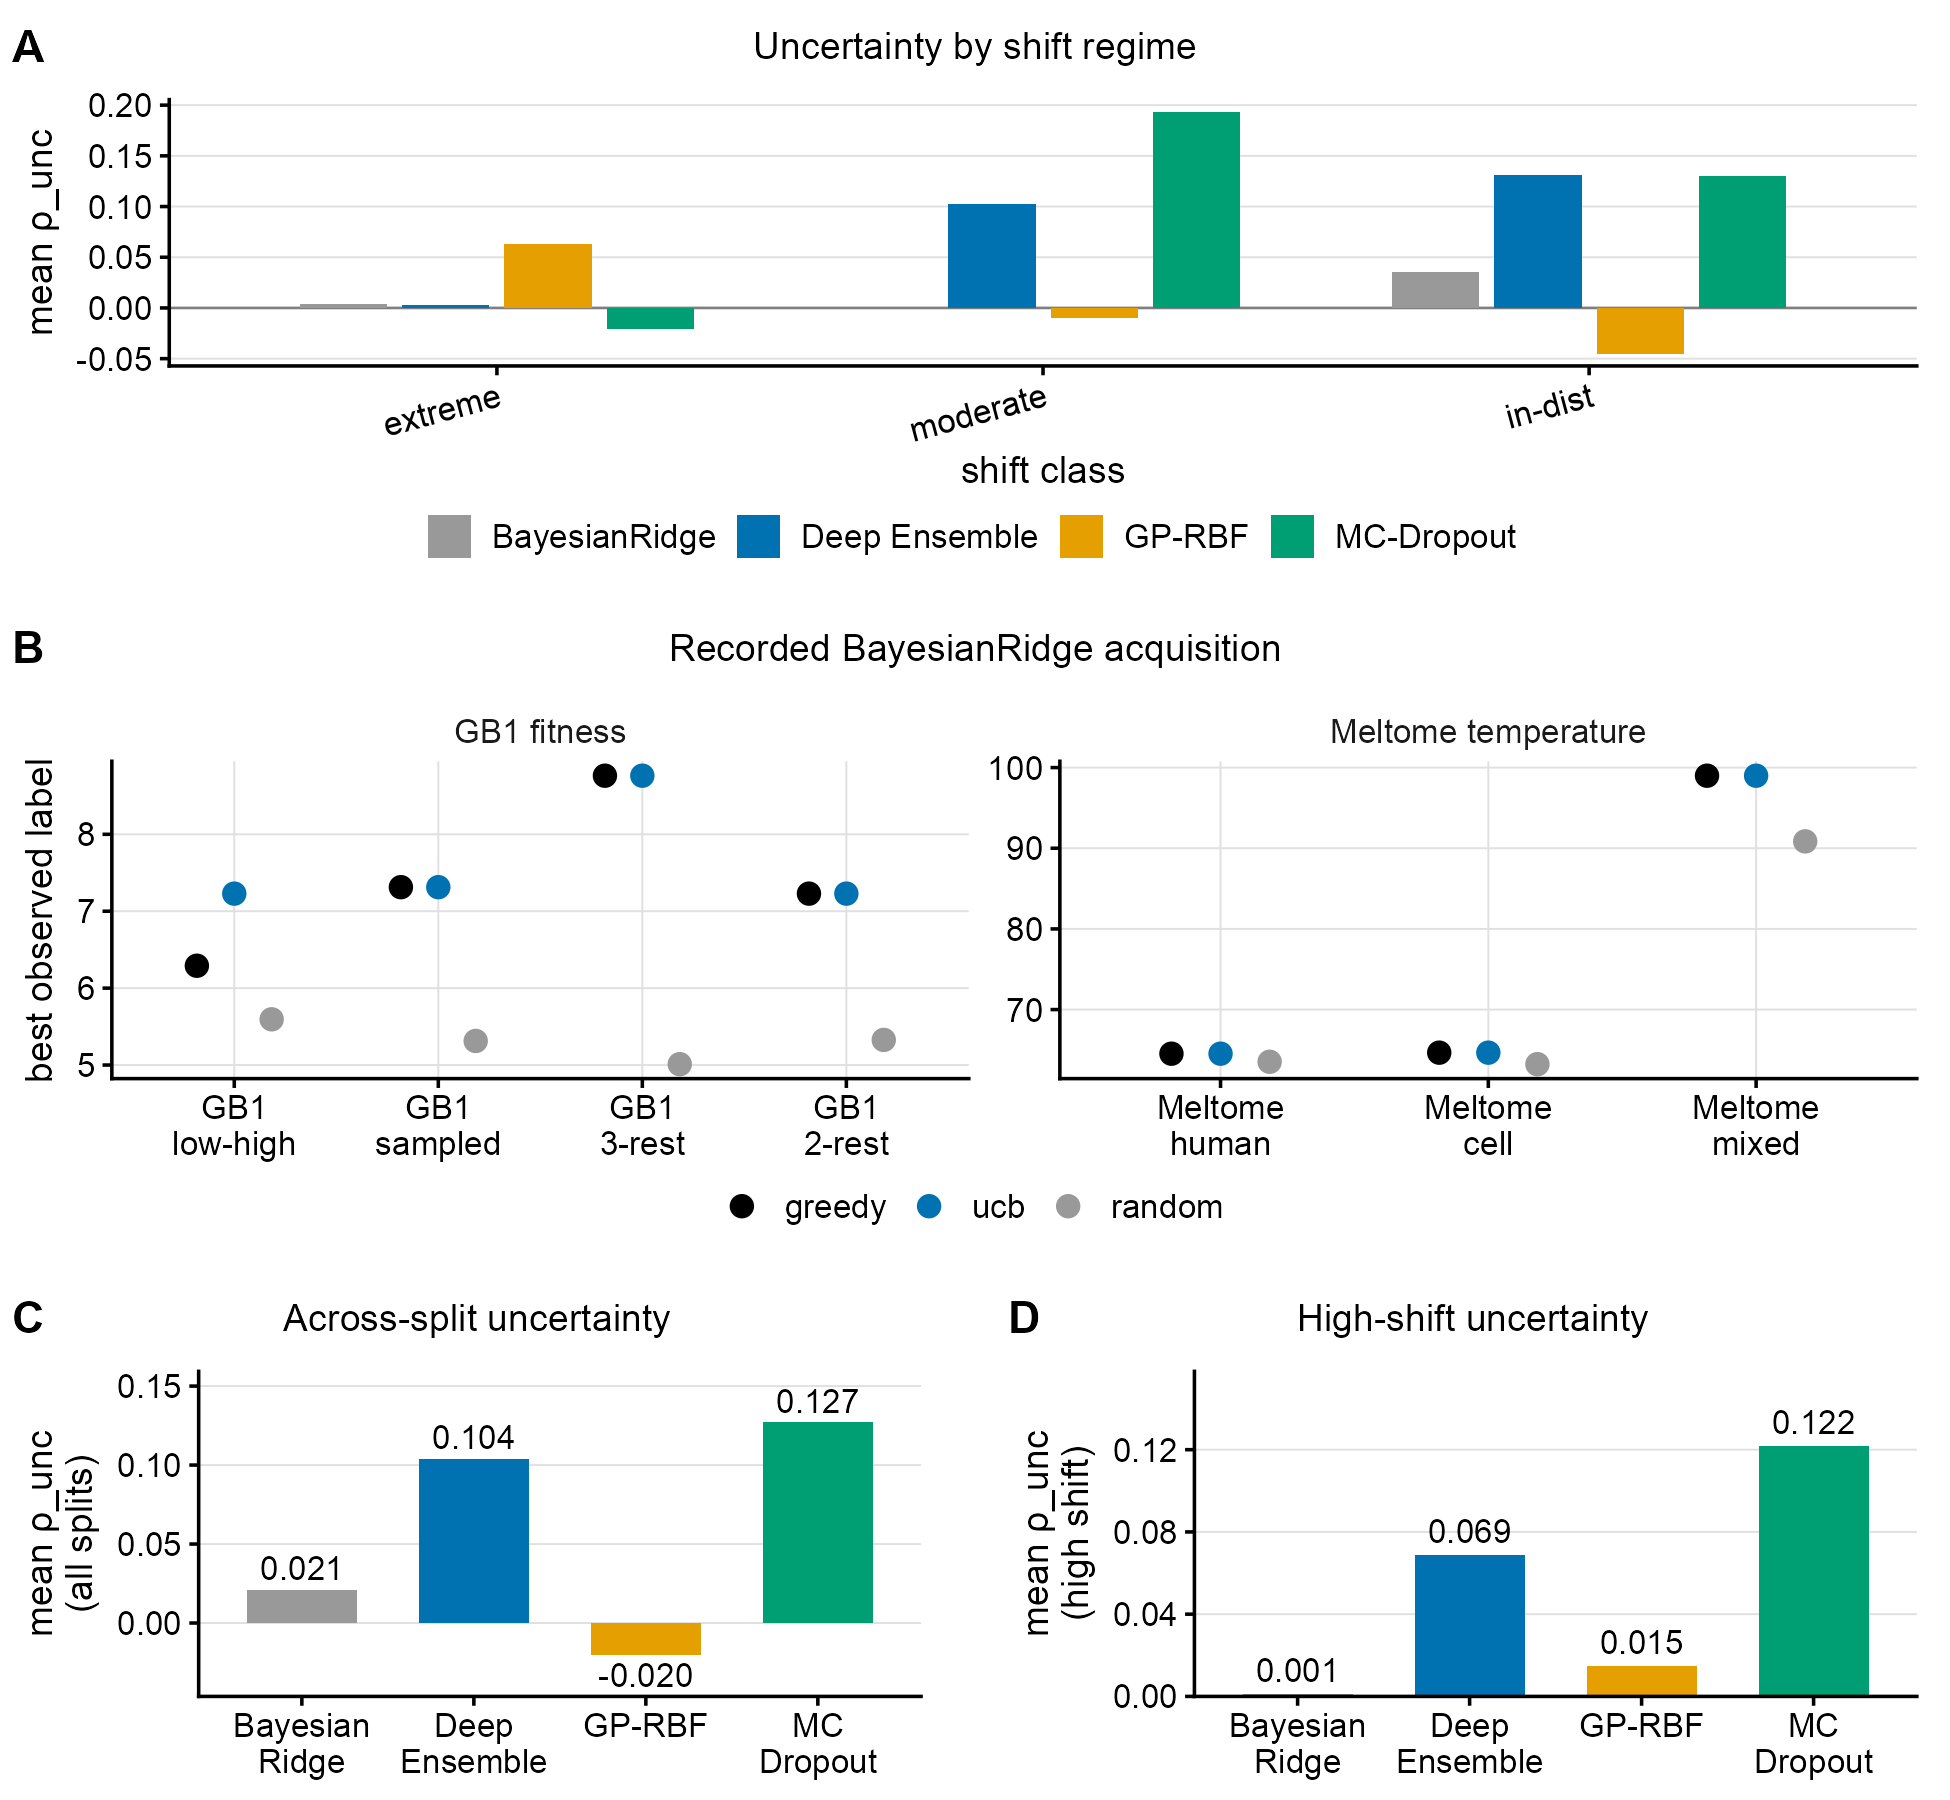
\includegraphics[width=\textwidth,height=0.82\textheight,keepaspectratio]{figures/F6_protein_uq.png}
\caption{\textbf{Fig 9$^\dagger$ (promoted SI S7 / ex-F6).} Learned UQ. (A)~Uncertainty--error correlation by shift. (B)~Method comparison. (C)~Acquisition (UCB vs greedy). (D)~Split-level summary.}\label{fig:f6}\end{figure}

\begin{figure}[p]\centering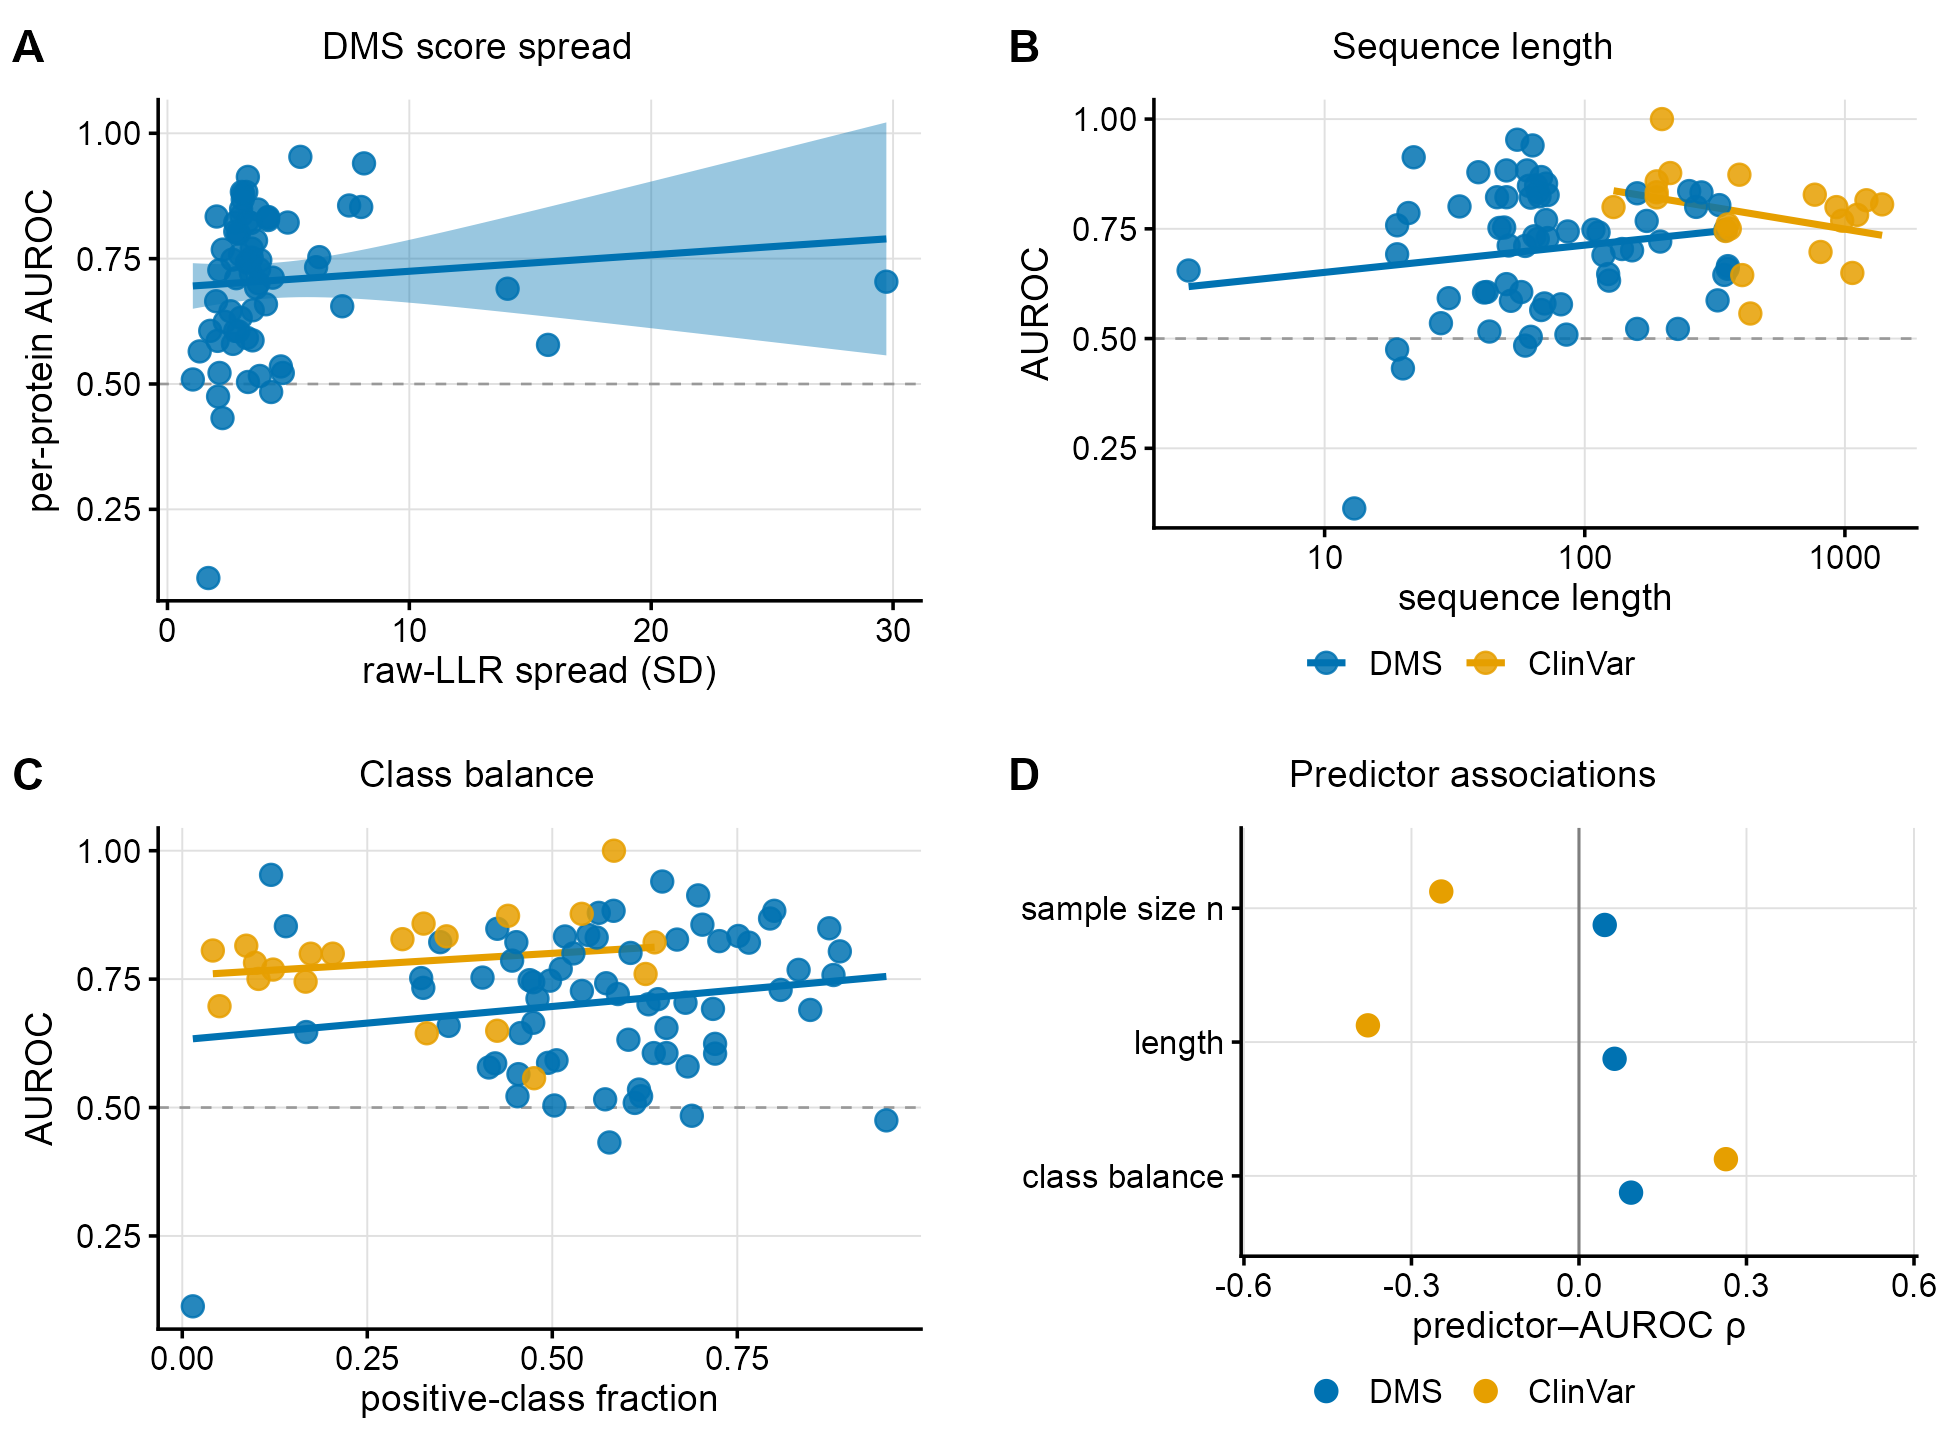
\includegraphics[width=\textwidth,height=0.82\textheight,keepaspectratio]{figures/F10_reliability_predictor.png}
\caption{\textbf{Fig 10$^\dagger$ (promoted SI S9 / ex-F10).} Reliability predictors. (A)~Score-spread vs AUROC. (B)~Length vs AUROC. (C)~Class balance vs AUROC. (D)~Cross-axis Spearman summary.}\label{fig:f10}\end{figure}

\end{document}
